% Part 1: Approximate the function in dataset (A) with a linear function.
% Part 1: Why is it not a good idea to use radial basis functions for dataset (A)?
% Part 2: Approximate the function in dataset (B) with a linear function.
% Part 3: Approximate the function in dataset (B) with a combination of radial functions.
% Discussed how and why you chose the values of L and ϵ for the radial basis functions?

For this task of approximating linear functions using least-squares minimization, we use the two datasets, (A) \texttt{linear\_function\_data.txt} and (B) \texttt{nonlinear\_function\_data.txt} provided to us. Each of them contains 1000 one-dimensional points each, with two columns: \textit{x} and \textit{f(x)}.

\begin{itemize}
    \item \textbf{First part}: \texttt{Approximating function in dataset (A) with a linear function}\\
    For dataset (A), containing 1000 points, we aim to approximate the underlying linear function. The linear model is represented by \textit{f$_{linear}$ = Ax}, where A is the matrix of coefficients. We used the function \texttt{least\_square\_minimization} employing \textit{scipy.linalg.lstsq} to find the matrix A. The original and the linear approximation of the data is shown in figure \ref{task5_1_1}. It can be seen that our linear function provides a highly accurate approximation of the data.

    \textbf{Using radial basis functions for approximating dataset (A):} Choosing radial basis functions for linear approximation is generally not a good idea because of the extra parameters and high computational overhead. Instead, linear models are capable, computationally efficient, and provide accurate representations for linear functions without the risk of overfitting.

\begin{figure}[H]
    \centering
    \begin{subfigure}{0.4\textwidth}
        \centering
        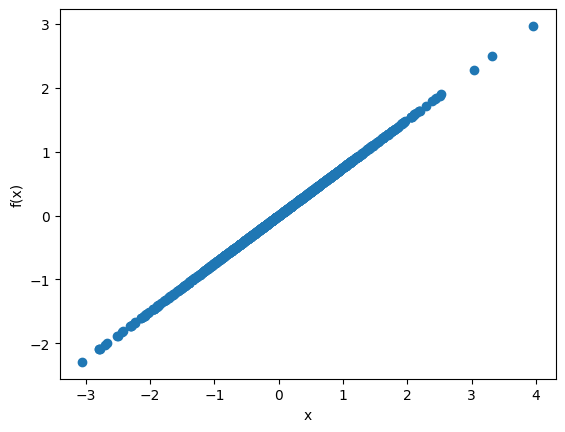
\includegraphics[width=\linewidth]{images/ex5task1_1Original.png}
        \caption{Original Dataset (A)}
        \label{task5_1Original}
    \end{subfigure}
    \begin{subfigure}{0.4\textwidth}
    \centering
        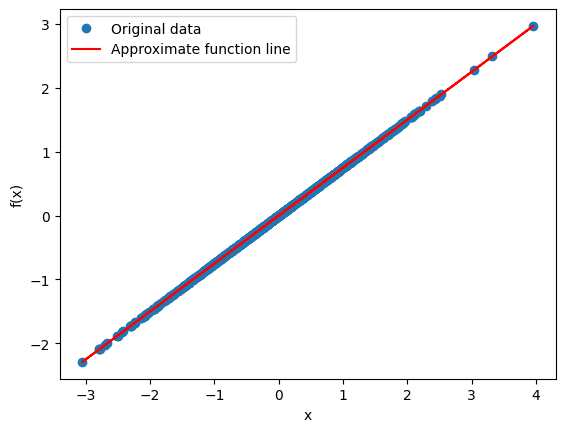
\includegraphics[width=\linewidth]{images/ex5task1_1Approximated.png}
        \caption{Linear Approximation of Dataset (A)}
        \label{task5_1Approximated}
    \end{subfigure}
    \caption{Original and approximated Dataset (A)}
    \label{task5_1_1}
\end{figure}

\item \textbf{Second part: }\texttt{Approximating the function in dataset (B) with a linear function}\\
The given dataset (B) is nonlinear as can be seen in figure \ref{task5_2Original}. Using the same linear approximation as in the previous task, we plotted the approximated function shown in figure \ref{task5_2Approximated}. A linear model can not properly approximate a non-linear dataset as can be seen by its inability to capture the dataset patterns.

\begin{figure}[H]
    \centering
    \begin{subfigure}{0.45\textwidth}
        \centering
        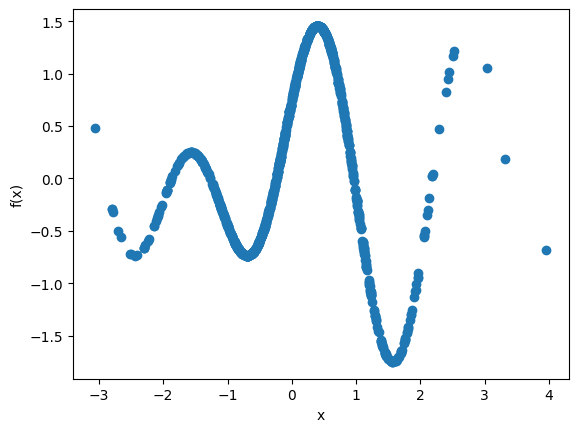
\includegraphics[width=\linewidth]{images/ex5task1_2Original.png}
        \caption{Original Dataset (B)}
        \label{task5_2Original}
    \end{subfigure}
    \begin{subfigure}{0.45\textwidth}
    \centering
        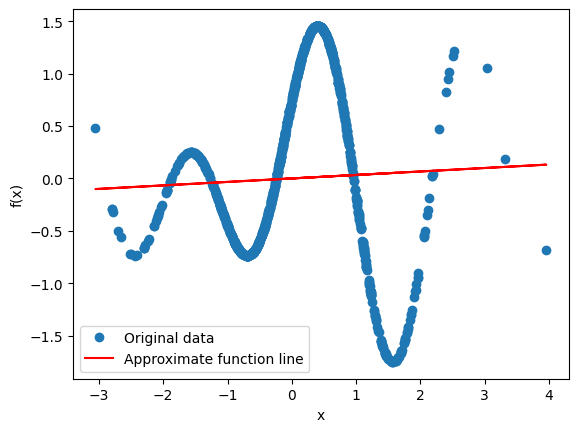
\includegraphics[width=\linewidth]{images/ex5task1_2.png}
        \caption{Linear Approximation of Dataset (B)}
        \label{task5_2Approximated}
    \end{subfigure}
    \caption{Original and approximated Dataset (B)}
    \label{task5_1_2}
\end{figure}

\item \textbf{Third part: }\texttt{Approximating the function in dataset(B) with a combination of radial functions}
For this section, we aim to approximate the non-linear function in dataset (B) with radial basis functions (RBFs). These basis functions provide greater flexibility to capture nonlinear relationships in the data. The challenge now lies in selecting the appropriate \textit{L} (number of centers or the number of functions) and the $\epsilon$ (width of basis functions). \\
\begin{itemize}
    \item \textbf{Selecting $\epsilon$:}
    Selecting \textit{L} to be equal to the number of data points will give us maximum accuracy but at the same time will be extremely computationally intensive. However, we can use a moderate number of functions to try and narrow down the values of $\epsilon$. So we first set the value of \textit{L} as 30 and try to fit the function to our data. We see in Fig. \ref{task5_1_3eps} that for values of $\epsilon$ greater than 1, the function approximation was pretty good. So we arbitrarily chose 2.0 as the $\epsilon$ value. 
    \begin{figure}[H]
    \centering
    \begin{subfigure}{\textwidth}
        \centering
        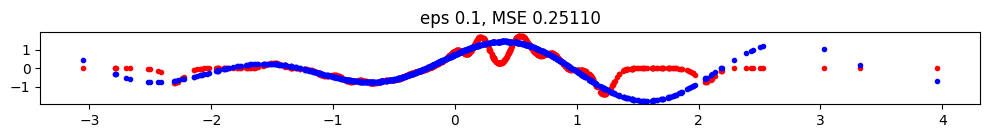
\includegraphics[width=0.6\linewidth]{images/epsilon0.1.png}
        \caption{$\epsilon=0.1$}
        \label{epsilon0_1}
    \end{subfigure}
    \begin{subfigure}{\textwidth}
    \centering
        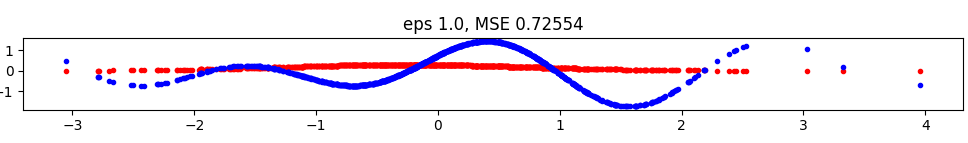
\includegraphics[width=0.6\linewidth]{images/epsilon1.0.png}
        \caption{$\epsilon=1.0$}
        \label{epsilon1}
    \end{subfigure}
    \begin{subfigure}{\textwidth}
    \centering
        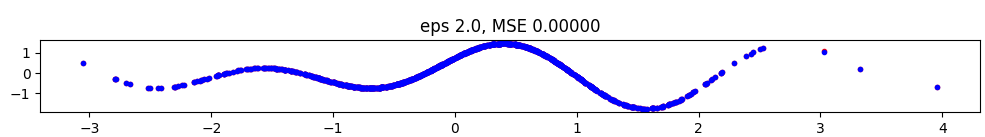
\includegraphics[width=0.6\linewidth]{images/epsilon2.0.png}
        \caption{$\epsilon=2.0$}
        \label{epsilon2}
    \end{subfigure}
    \caption{Function approximation for different values of $\epsilon$}
    \label{task5_1_3eps}
\end{figure}
    \item \textbf{Selecting \textit{L}:}
    Now, using this $\epsilon$, we again tried to approximate the function by choosing different values of \textit{L} between 5-20. Looking at the result, we found that a value of 12 (Fig. \ref{L12}) captured the function pretty well without overfitting. Thus, we chose the values of \textit{L} to be 20 and $\epsilon$ to be 2.0.
    \begin{figure}[H]
    \centering
    \begin{subfigure}{\textwidth}
        \centering
        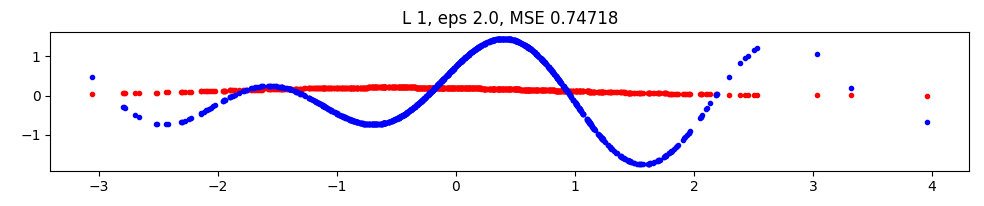
\includegraphics[width=0.6\linewidth]{images/Lvalues1.png}
        \caption{L=1}
        \label{L1}
    \end{subfigure}
    \begin{subfigure}{\textwidth}
    \centering
        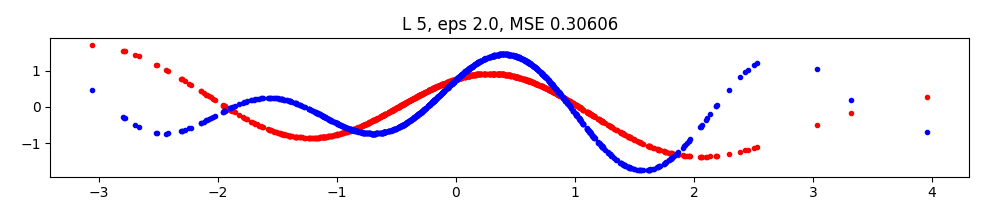
\includegraphics[width=0.6\linewidth]{images/Lvalues5.png}
        \caption{L=5}
        \label{L5}
    \end{subfigure}
    \begin{subfigure}{\textwidth}
    \centering
        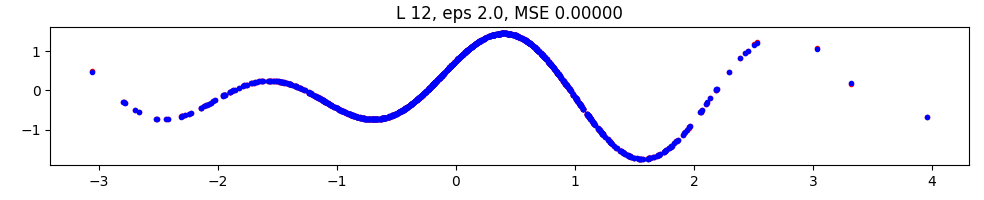
\includegraphics[width=0.6\linewidth]{images/Lvalues10.png}
        \caption{L=12}
        \label{L12}
    \end{subfigure}
    \caption{Function approximation for different values of \textit{L}}
    \label{task5_1_3L}
\end{figure}
\end{itemize}

The final approximated function can be seen in figure \ref{ApproximatedB} with \textit{L}=10 and $\epsilon$=2.0.

\begin{figure}[H]
    \centering
    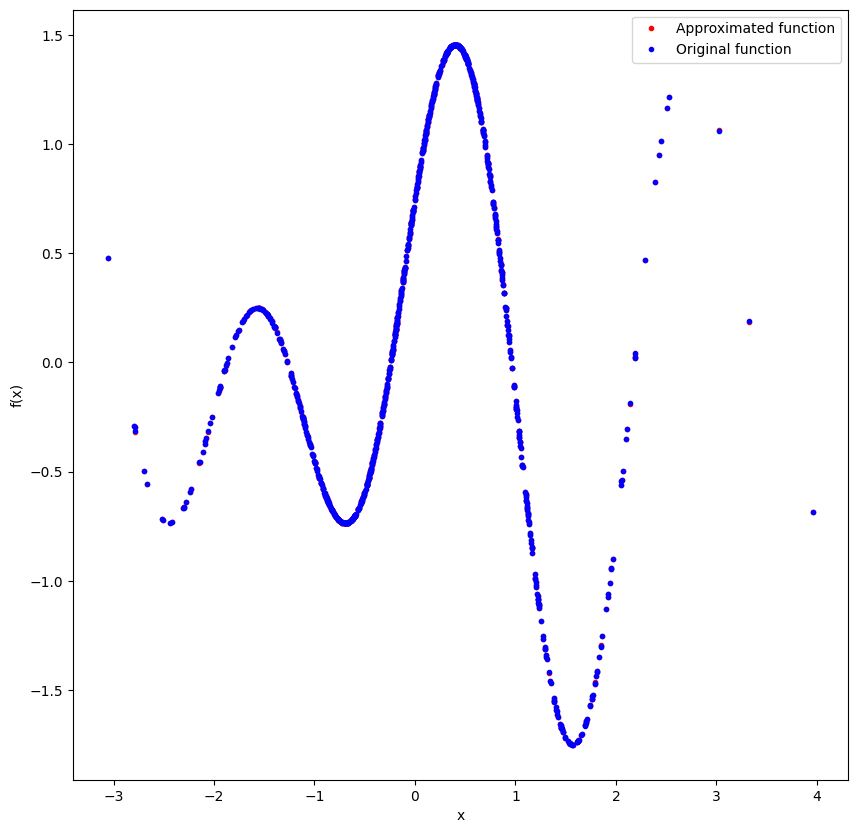
\includegraphics[width=0.6\linewidth]{images/Ex5task1_3.png}
    \caption{Approximated function for Dataset (B) using radial basis functions}
    \label{ApproximatedB}
\end{figure}



\end{itemize}